% English figures of the final report (one figure per page).
% Build: pdflatex report_figures.tex ; then render each page to PNG (see report/README or the build note in the report).
\documentclass[border=6pt,multi=figpage]{standalone}
\usepackage[T5]{fontenc}
\usepackage[utf8]{inputenc}
\usepackage{lmodern}
\usepackage{tikz}
\usetikzlibrary{arrows.meta,positioning,fit,backgrounds,calc,shapes.geometric,shapes.multipart}
\usepackage{pgfplots}
\pgfplotsset{compat=1.17}
\pgfkeys{/pgf/number format/.cd,use period,1000 sep={\mathord{,}}}
\definecolor{bkblue}{HTML}{1E4E79}
\definecolor{bkorange}{HTML}{C8742E}
\definecolor{bkgreen}{HTML}{1F7A3A}
\definecolor{bkgray}{HTML}{8A97A6}
\newenvironment{figpage}{}{}
\begin{document}

% ---------------------------------------------------------------- 1. solution pipeline
\begin{figpage}
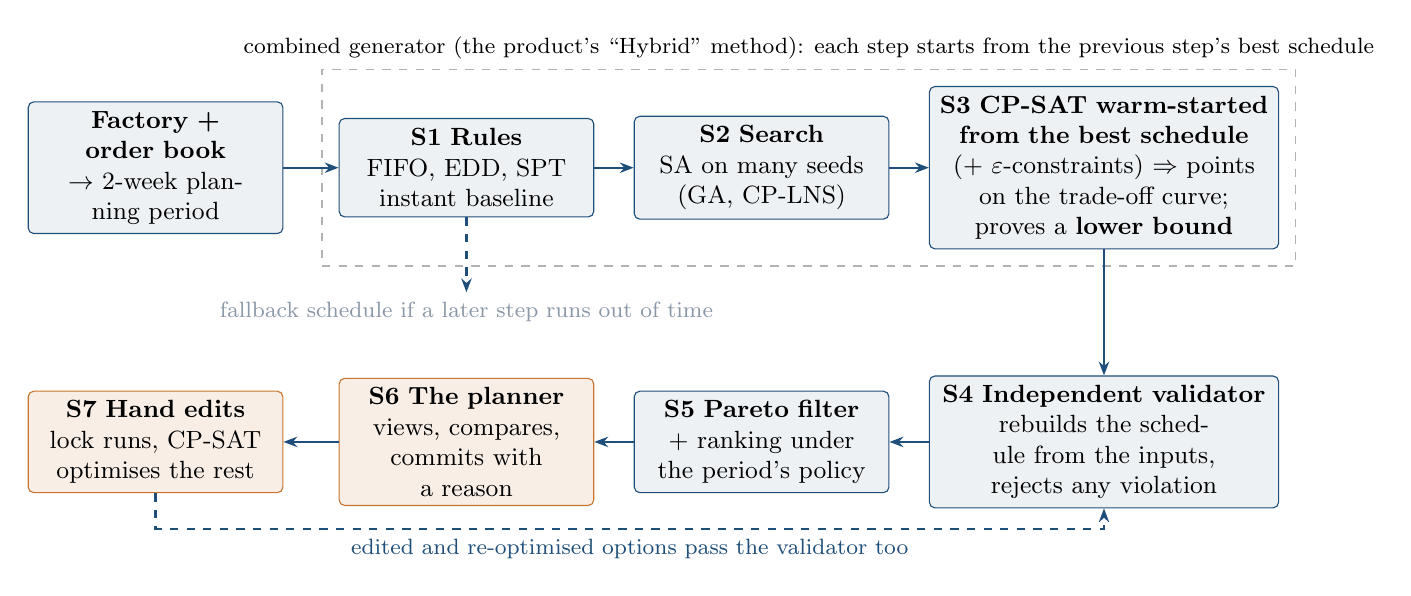
\begin{tikzpicture}[font=\small,
  b/.style={draw=bkblue,fill=bkblue!8,rounded corners=2pt,align=center,minimum height=1.25cm,text width=3.0cm},
  h/.style={b,draw=bkorange,fill=bkorange!12},
  a/.style={-{Stealth[length=5pt]},bkblue,thick}, node distance=0.5cm]
  \node[b] (in) {\textbf{Factory + order book}\\$\to$ 2-week planning period};
  \node[b,right=0.7cm of in] (b1) {\textbf{S1 Rules}\\FIFO, EDD, SPT\\instant baseline};
  \node[b,right=of b1] (b2) {\textbf{S2 Search}\\SA on many seeds\\(GA, CP-LNS)};
  \node[b,right=of b2,text width=4.2cm] (b3) {\textbf{S3 CP-SAT warm-started from the best schedule} (+ $\varepsilon$-constraints) $\Rightarrow$ points on the trade-off curve; proves a \textbf{lower bound}};
  \node[b,below=1.6cm of b3,text width=4.2cm] (b4) {\textbf{S4 Independent validator}\\rebuilds the schedule from the inputs, rejects any violation};
  \node[b,left=of b4] (b5) {\textbf{S5 Pareto filter}\\+ ranking under the period's policy};
  \node[h,left=of b5] (b6) {\textbf{S6 The planner}\\views, compares,\\commits with a reason};
  \node[h,left=0.7cm of b6] (b7) {\textbf{S7 Hand edits}\\lock runs, CP-SAT\\optimises the rest};
  \draw[a] (in)--(b1); \draw[a] (b1)--(b2); \draw[a] (b2)--(b3);
  \draw[a] (b3)--(b4); \draw[a] (b4)--(b5); \draw[a] (b5)--(b6); \draw[a] (b6)--(b7);
  \draw[a,dashed] (b7.south) -- ++(0,-0.45) -| node[pos=0.25,below,font=\footnotesize]{edited and re-optimised options pass the validator too} (b4.south);
  \draw[a,dashed] (b1.south) -- ++(0,-0.95) node[below,font=\footnotesize,align=center,text=bkgray]{fallback schedule if a later step runs out of time};
  \begin{scope}[on background layer]
    \node[fit=(b1)(b3),draw=gray!60,dashed,inner sep=6pt,label={[font=\footnotesize]above:combined generator (the product's ``Hybrid'' method): each step starts from the previous step's best schedule}] {};
  \end{scope}
\end{tikzpicture}
\end{figpage}

% ---------------------------------------------------------------- 2. 3-day trade-off
\begin{figpage}
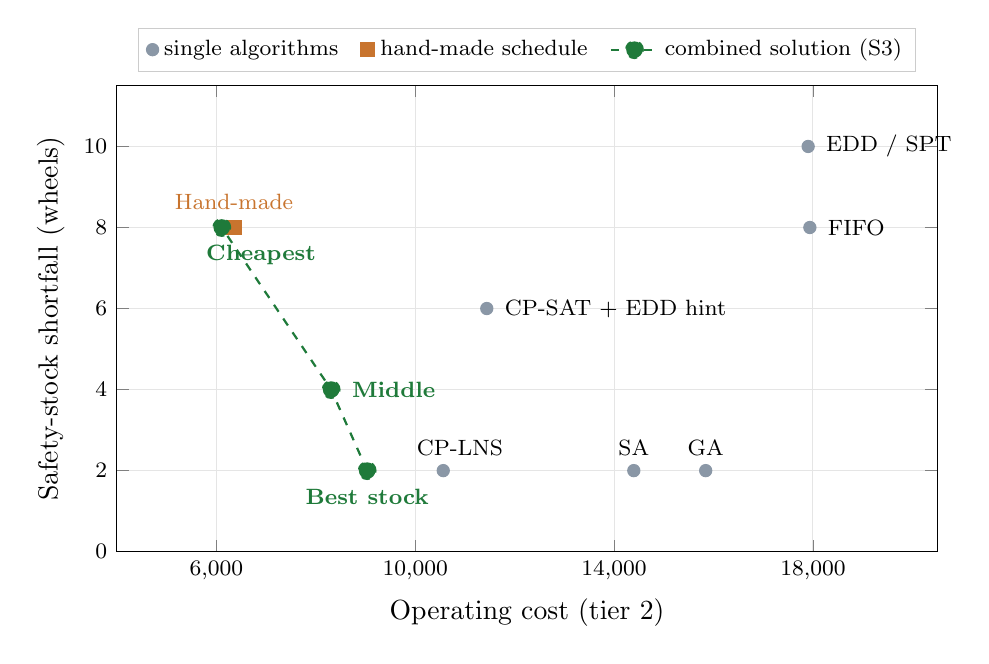
\begin{tikzpicture}
\begin{axis}[width=12cm,height=7.5cm,
  xlabel={Operating cost (tier 2)},ylabel={Safety-stock shortfall (wheels)},
  xmin=4000,xmax=20500,ymin=0,ymax=11.5,
  tick label style={font=\footnotesize},
  xtick={6000,10000,14000,18000}, scaled x ticks=false,
  grid=major,grid style={gray!20},
  legend columns=3,
  legend style={font=\footnotesize,at={(0.5,1.03)},anchor=south,draw=gray!40,/tikz/every even column/.append style={column sep=6pt}},
  clip=false]
\addplot[only marks,mark=*,mark size=2.2pt,color=bkgray] coordinates
  {(10564,2) (14397,2) (15843,2) (11440,6) (17938,8) (17904,10)};
\addplot[only marks,mark=square*,mark size=2.6pt,color=bkorange] coordinates {(6356,8)};
\addplot[thick,dashed,mark=*,mark size=3pt,color=bkgreen] coordinates {(9034,2) (8310,4) (6110,8)};
\legend{single algorithms,hand-made schedule,combined solution (S3)}
\begin{scope}[font=\footnotesize]
  \node[anchor=south,yshift=2pt] at (axis cs:10900,2) {CP-LNS};
  \node[anchor=south,yshift=2pt] at (axis cs:14397,2) {SA};
  \node[anchor=south,yshift=2pt] at (axis cs:15843,2) {GA};
  \node[anchor=west,xshift=3pt] at (axis cs:11440,6) {CP-SAT + EDD hint};
  \node[anchor=west,xshift=3pt] at (axis cs:17938,8) {FIFO};
  \node[anchor=west,xshift=3pt] at (axis cs:17904,10) {EDD / SPT};
  \node[anchor=south,yshift=3pt,text=bkorange] at (axis cs:6356,8) {Hand-made};
  \node[anchor=north,yshift=-3pt,text=bkgreen,font=\footnotesize\bfseries] at (axis cs:9034,2) {Best stock};
  \node[anchor=west,xshift=4pt,text=bkgreen,font=\footnotesize\bfseries] at (axis cs:8310,4) {Middle};
  \node[anchor=north west,yshift=-3pt,text=bkgreen,font=\footnotesize\bfseries] at (axis cs:5600,8) {Cheapest};
\end{scope}
\end{axis}
\end{tikzpicture}
\end{figpage}

% ---------------------------------------------------------------- 3. 2-week CP-SAT from SA
\begin{figpage}
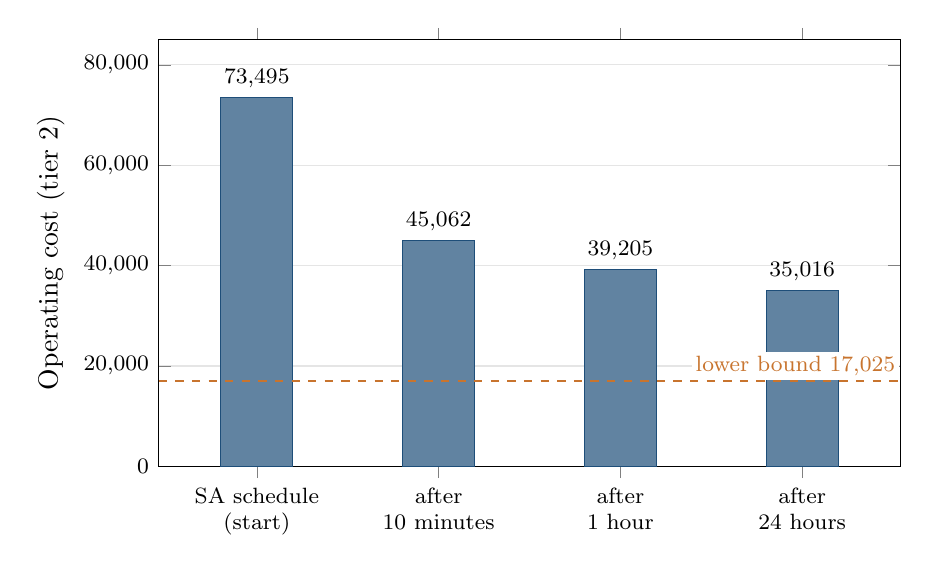
\begin{tikzpicture}
\begin{axis}[width=11cm,height=7cm,ybar,bar width=26pt,
  ymin=0,ymax=85000,
  symbolic x coords={SA,10',1h,24h},xtick=data,
  xticklabels={{SA schedule\\(start)},{after\\10 minutes},{after\\1 hour},{after\\24 hours}},
  xticklabel style={align=center,font=\footnotesize},
  ylabel={Operating cost (tier 2)},
  tick label style={font=\footnotesize},scaled y ticks=false,
  nodes near coords,every node near coord/.append style={font=\footnotesize},
  grid=major,ymajorgrids=true,xmajorgrids=false,grid style={gray!20},
  enlarge x limits=0.18]
\addplot[fill=bkblue!70,draw=bkblue] coordinates {(SA,73495) (10',45062) (1h,39205) (24h,35016)};
\draw[dashed,thick,bkorange] (rel axis cs:0,0.2003) -- (rel axis cs:1,0.2003)
  node[pos=1,above left,font=\footnotesize,text=bkorange,fill=white,inner sep=1.5pt] {lower bound 17,025};
\end{axis}
\end{tikzpicture}
\end{figpage}

% ---------------------------------------------------------------- 4. use-case diagram
\begin{figpage}
\begin{tikzpicture}[font=\small,
  uc/.style={ellipse,draw=bkblue,fill=bkblue!6,minimum width=5.6cm,minimum height=0.72cm,inner sep=1pt,align=center},
  ucv/.style={uc,draw=bkorange,fill=bkorange!10,minimum width=3.4cm},
  inc/.style={-{Stealth[length=4pt]},dashed,bkgray}]
  \def\actor#1#2{%
    \begin{scope}[shift={#1}]
      \draw[thick] (0,0.55) circle (0.22);
      \draw[thick] (0,0.33)--(0,-0.25) (-0.32,0.12)--(0.32,0.12) (0,-0.25)--(-0.25,-0.7) (0,-0.25)--(0.25,-0.7);
      \node[below,align=center,font=\small\bfseries] at (0,-0.75) {#2};
    \end{scope}}
  \foreach \i/\t in {1/UC-01 Maintain the factory set-up,2/UC-02 Manage the order book,3/UC-03 Prepare a planning period,
                     4/UC-04 Generate schedule options,5/UC-05 Compare and inspect options,6/UC-06 Edit by hand + optimise the rest,
                     7/UC-07 Commit a schedule,8/UC-08 Execute: work orders,9/UC-09 Reschedule after an incident,
                     10/UC-10 Create a what-if variant,11/UC-11 Close and roll over a period,12/UC-12 Analyse runs and decisions}
    \node[uc] (u\i) at (0,-\i*0.92) {\t};
  \node[ucv] (val) at (7.4,-6*0.92) {Validate a schedule\\(independent validator)};
  \begin{scope}[on background layer]
    \node[draw=gray!70,rounded corners=4pt,fit=(u1)(u12)(val),inner sep=10pt,
          label={[font=\small\bfseries]above:Production scheduling system (PlanWise)}] (sys) {};
  \end{scope}
  \actor{(-5.6,-3.6)}{Planner\\(operator role)}
  \actor{(-5.6,-9.6)}{Manager\\(reader role)}
  \foreach \i in {1,...,12} \draw (-5.25,-3.2) -- (u\i.west);
  \foreach \i in {5,8,12} \draw[bkorange] (-5.25,-9.2) -- (u\i.west);
  \foreach \i in {4,6,9} \draw[inc] (u\i.east) -- (val.west);
  \node[font=\scriptsize,text=bkgray,fill=white,inner sep=1pt] at (4.6,-5.29) {«include»};
\end{tikzpicture}
\end{figpage}

% ---------------------------------------------------------------- 5. architecture
\begin{figpage}
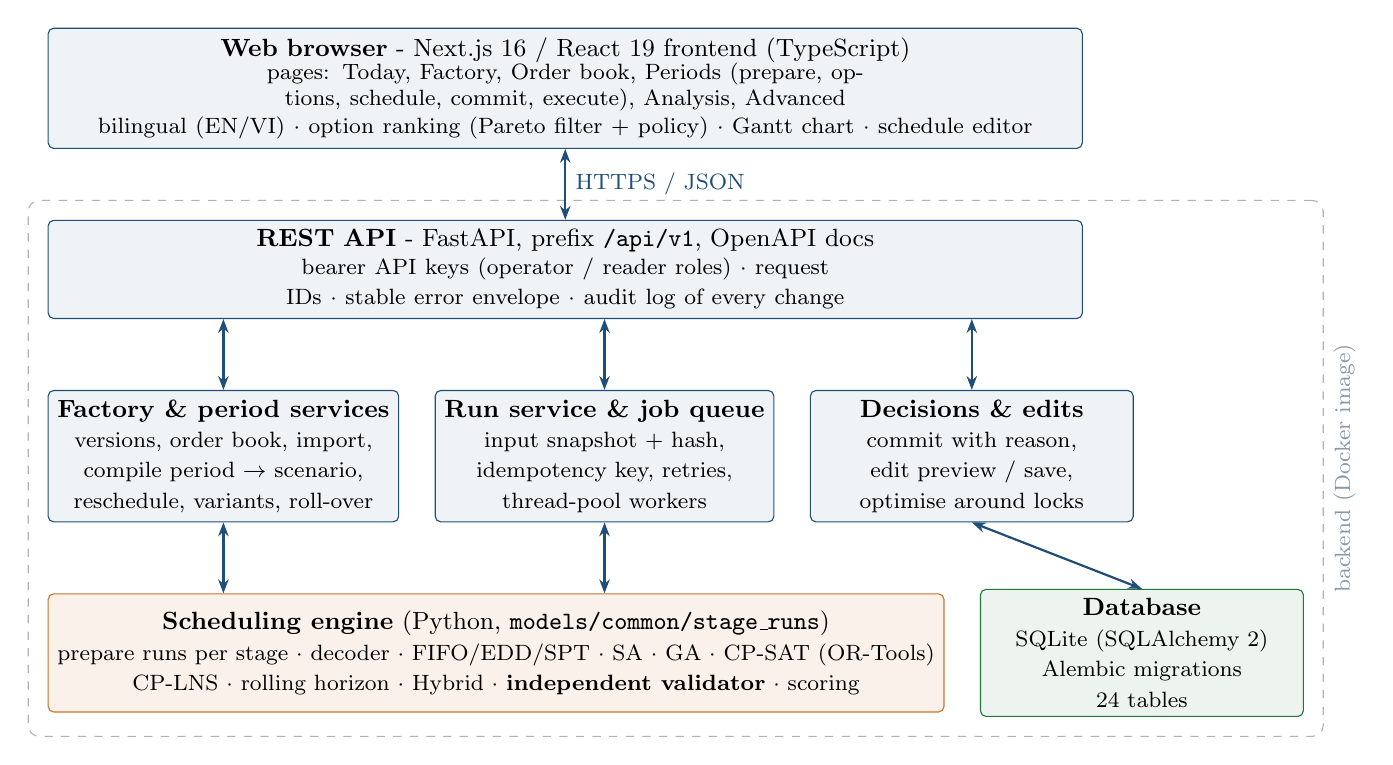
\begin{tikzpicture}[font=\small,
  box/.style={draw=bkblue,fill=bkblue!7,rounded corners=2pt,align=center,minimum height=1.0cm},
  layer/.style={draw=gray!60,dashed,rounded corners=4pt,inner sep=7pt},
  a/.style={{Stealth[length=5pt]}-{Stealth[length=5pt]},bkblue,thick}]
  % client
  \node[box,text width=12.9cm] (ui) at (0,0) {\textbf{Web browser} - Next.js 16 / React 19 frontend (TypeScript)\\[-1pt]\footnotesize pages: Today, Factory, Order book, Periods (prepare, options, schedule, commit, execute), Analysis, Advanced\\[-1pt]\footnotesize bilingual (EN/VI) $\cdot$ option ranking (Pareto filter + policy) $\cdot$ Gantt chart $\cdot$ schedule editor};
  % api
  \node[box,text width=12.9cm,below=0.9cm of ui] (api) {\textbf{REST API} - FastAPI, prefix \texttt{/api/v1}, OpenAPI docs\\[-1pt]\footnotesize bearer API keys (operator / reader roles) $\cdot$ request IDs $\cdot$ stable error envelope $\cdot$ audit log of every change};
  % services
  \node[box,minimum width=4.1cm,minimum height=1.55cm,below=0.9cm of api.south west,anchor=north west] (svc1) {\textbf{Factory \& period services}\\\footnotesize versions, order book, import,\\\footnotesize compile period $\to$ scenario,\\\footnotesize reschedule, variants, roll-over};
  \node[box,minimum width=4.1cm,minimum height=1.55cm,right=0.45cm of svc1] (svc2) {\textbf{Run service \& job queue}\\\footnotesize input snapshot + hash,\\\footnotesize idempotency key, retries,\\\footnotesize thread-pool workers};
  \node[box,minimum width=4.1cm,minimum height=1.55cm,right=0.45cm of svc2] (svc3) {\textbf{Decisions \& edits}\\\footnotesize commit with reason,\\\footnotesize edit preview / save,\\\footnotesize optimise around locks};
  % engine
  \node[box,draw=bkorange,fill=bkorange!10,minimum width=8.65cm,minimum height=1.5cm,below=0.9cm of svc1.south west,anchor=north west] (eng) {\textbf{Scheduling engine} (Python, \texttt{models/common/stage\_runs})\\\footnotesize prepare runs per stage $\cdot$ decoder $\cdot$ FIFO/EDD/SPT $\cdot$ SA $\cdot$ GA $\cdot$ CP-SAT (OR-Tools)\\\footnotesize CP-LNS $\cdot$ rolling horizon $\cdot$ Hybrid $\cdot$ \textbf{independent validator} $\cdot$ scoring};
  \node[box,draw=bkgreen,fill=bkgreen!8,minimum width=4.1cm,minimum height=1.5cm,right=0.45cm of eng] (db) {\textbf{Database}\\\footnotesize SQLite (SQLAlchemy 2)\\\footnotesize Alembic migrations\\\footnotesize 24 tables};
  \draw[a] (ui) -- node[right,font=\footnotesize]{HTTPS / JSON} (api);
  \foreach \s in {svc1,svc2,svc3} \draw[a] (api.south -| \s.north) -- (\s.north);
  \draw[a] (svc1.south) -- (svc1.south |- eng.north);
  \draw[a] (svc2.south) -- (svc2.south |- eng.north);
  \draw[a] (svc3.south) -- (db.north);
  \begin{scope}[on background layer]
    \node[layer,fit=(api)(svc1)(svc3)(eng)(db),label={[font=\footnotesize,text=bkgray]right:\rotatebox{90}{backend (Docker image)}}] {};
  \end{scope}
\end{tikzpicture}
\end{figpage}

% ---------------------------------------------------------------- 6. sequence: generate options
\begin{figpage}
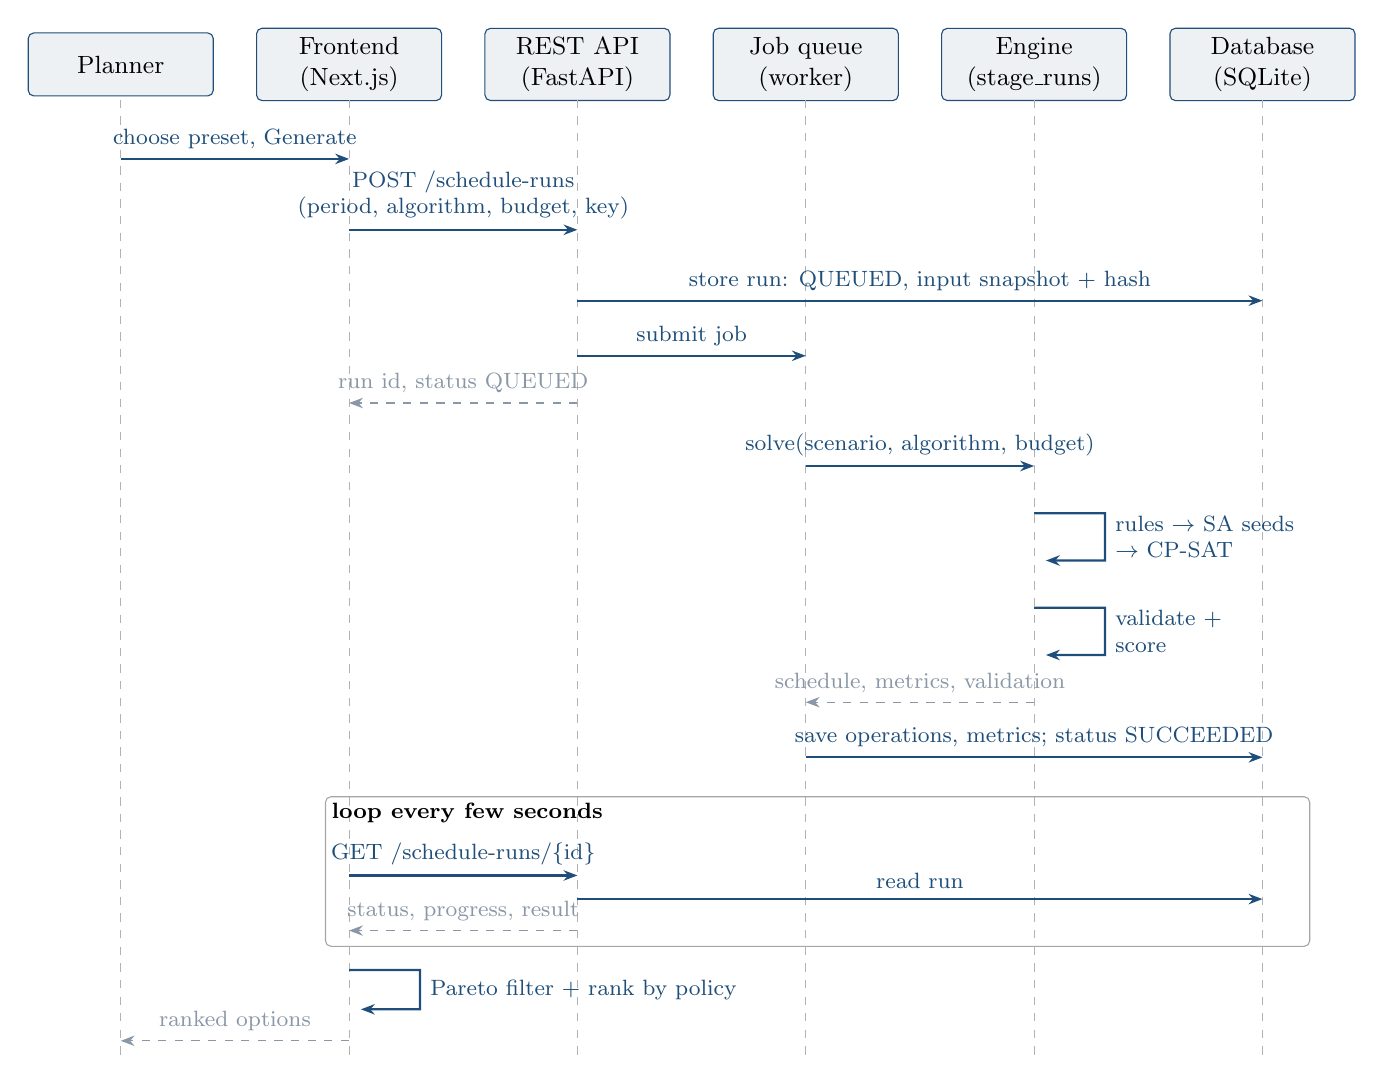
\begin{tikzpicture}[font=\small,
  head/.style={draw=bkblue,fill=bkblue!8,rounded corners=2pt,minimum width=2.35cm,minimum height=0.8cm,align=center},
  msg/.style={-{Stealth[length=5pt]},thick,bkblue},
  ret/.style={-{Stealth[length=5pt]},dashed,bkgray},
  act/.style={fill=white,draw=bkblue,minimum width=0.22cm}]
  \foreach \x/\n/\t in {0/pl/Planner,2.9/fe/Frontend\\(Next.js),5.8/api/REST API\\(FastAPI),8.7/q/Job queue\\(worker),11.6/en/Engine\\(stage\_runs),14.5/db/Database\\(SQLite)}
    { \node[head] (\n) at (\x,0) {\t}; \draw[gray!60,dashed] (\x,-0.45) -- (\x,-12.6); }
  \def\m#1#2#3#4{\draw[msg] (#1,-#3) -- node[above,font=\footnotesize,align=center]{#4} (#2,-#3);}
  \def\r#1#2#3#4{\draw[ret] (#1,-#3) -- node[above,font=\footnotesize,align=center]{#4} (#2,-#3);}
  \m{0}{2.9}{1.2}{choose preset, Generate}
  \m{2.9}{5.8}{2.1}{POST /schedule-runs\\(period, algorithm, budget, key)}
  \m{5.8}{14.5}{3.0}{store run: QUEUED, input snapshot + hash}
  \m{5.8}{8.7}{3.7}{submit job}
  \r{5.8}{2.9}{4.3}{run id, status QUEUED}
  \m{8.7}{11.6}{5.1}{solve(scenario, algorithm, budget)}
  \draw[msg] (11.6,-5.7) -- ++(0.9,0) -- ++(0,-0.6) node[right,pos=0.5,font=\footnotesize,align=left]{rules $\to$ SA seeds\\$\to$ CP-SAT} -- (11.75,-6.3);
  \draw[msg] (11.6,-6.9) -- ++(0.9,0) -- ++(0,-0.6) node[right,pos=0.5,font=\footnotesize,align=left]{validate +\\score} -- (11.75,-7.5);
  \r{11.6}{8.7}{8.1}{schedule, metrics, validation}
  \m{8.7}{14.5}{8.8}{save operations, metrics; status SUCCEEDED}
  \draw[gray!70,rounded corners=2pt] (2.6,-9.3) rectangle (15.1,-11.2);
  \node[anchor=north west,font=\footnotesize\bfseries,inner sep=2pt] at (2.6,-9.3) {loop every few seconds};
  \m{2.9}{5.8}{10.3}{GET /schedule-runs/\{id\}}
  \m{5.8}{14.5}{10.6}{read run}
  \r{5.8}{2.9}{11.0}{status, progress, result}
  \draw[msg] (2.9,-11.5) -- ++(0.9,0) -- ++(0,-0.5) node[right,pos=0.5,font=\footnotesize]{Pareto filter + rank by policy} -- (3.05,-12.0);
  \r{2.9}{0}{12.4}{ranked options}
\end{tikzpicture}
\end{figpage}

% ---------------------------------------------------------------- 7. period life cycle
\begin{figpage}
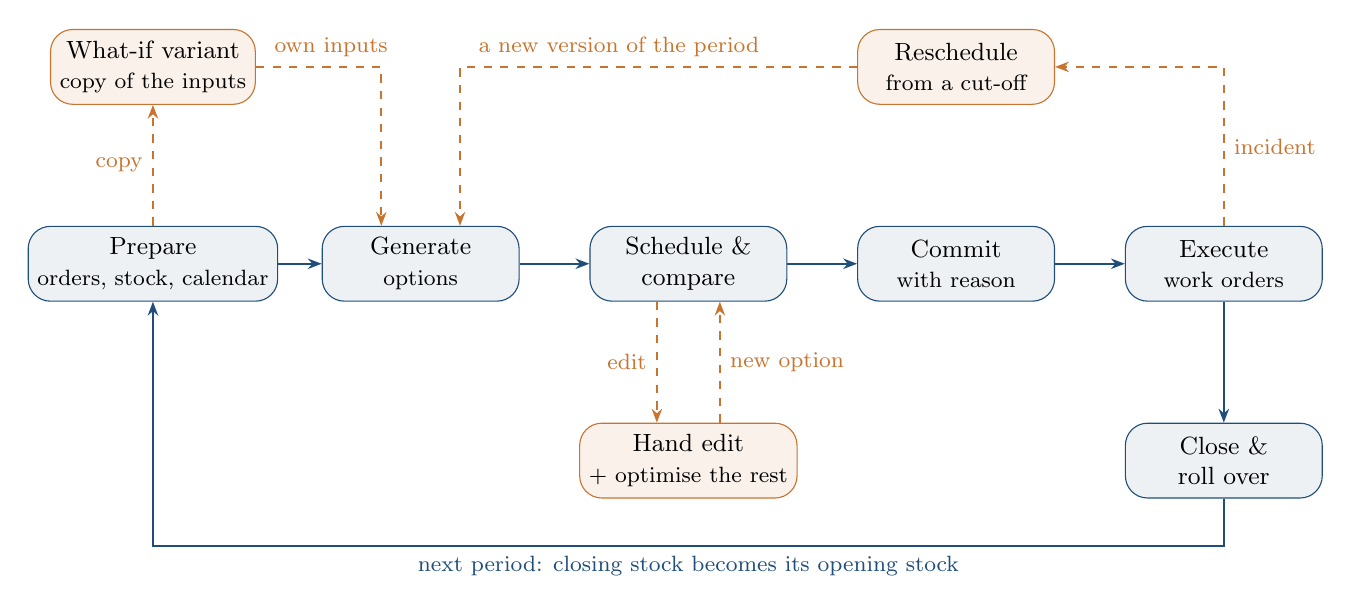
\begin{tikzpicture}[font=\small,
  st/.style={draw=bkblue,fill=bkblue!8,rounded corners=8pt,minimum width=2.5cm,minimum height=0.95cm,align=center},
  side/.style={st,draw=bkorange,fill=bkorange!10},
  a/.style={-{Stealth[length=5pt]},thick,bkblue},
  b/.style={-{Stealth[length=5pt]},dashed,bkorange,thick}]
  \node[st] (prep) at (0,0) {Prepare\\\footnotesize orders, stock, calendar};
  \node[st] (gen) at (3.4,0) {Generate\\\footnotesize options};
  \node[st] (cmp) at (6.8,0) {Schedule \&\\compare};
  \node[st] (com) at (10.2,0) {Commit\\\footnotesize with reason};
  \node[st] (exe) at (13.6,0) {Execute\\\footnotesize work orders};
  \node[st] (clo) at (13.6,-2.5) {Close \&\\roll over};
  \node[side] (edit) at (6.8,-2.5) {Hand edit\\\footnotesize + optimise the rest};
  \node[side] (var) at (0,2.5) {What-if variant\\\footnotesize copy of the inputs};
  \node[side] (res) at (10.2,2.5) {Reschedule\\\footnotesize from a cut-off};
  \draw[a] (prep)--(gen); \draw[a] (gen)--(cmp); \draw[a] (cmp)--(com); \draw[a] (com)--(exe); \draw[a] (exe)--(clo);
  \draw[a] (clo.south) -- ++(0,-0.6) -| node[pos=0.25,below,font=\footnotesize]{next period: closing stock becomes its opening stock} (prep.south);
  \draw[b] ([xshift=-4mm]cmp.south) -- node[left,font=\footnotesize]{edit} ([xshift=-4mm]edit.north);
  \draw[b] ([xshift=4mm]edit.north) -- node[right,font=\footnotesize]{new option} ([xshift=4mm]cmp.south);
  \draw[b] (exe.north) |- node[pos=0.25,right,font=\footnotesize]{incident} (res.east);
  \draw[b] (res.west) -| node[pos=0.3,above,font=\footnotesize]{a new version of the period} ([xshift=5mm]gen.north);
  \draw[b] (prep.north) -- node[left,font=\footnotesize]{copy} (var.south);
  \draw[b] (var.east) -| node[pos=0.3,above,font=\footnotesize]{own inputs} ([xshift=-5mm]gen.north);
\end{tikzpicture}
\end{figpage}

% ---------------------------------------------------------------- 8. data model (core tables)
\begin{figpage}
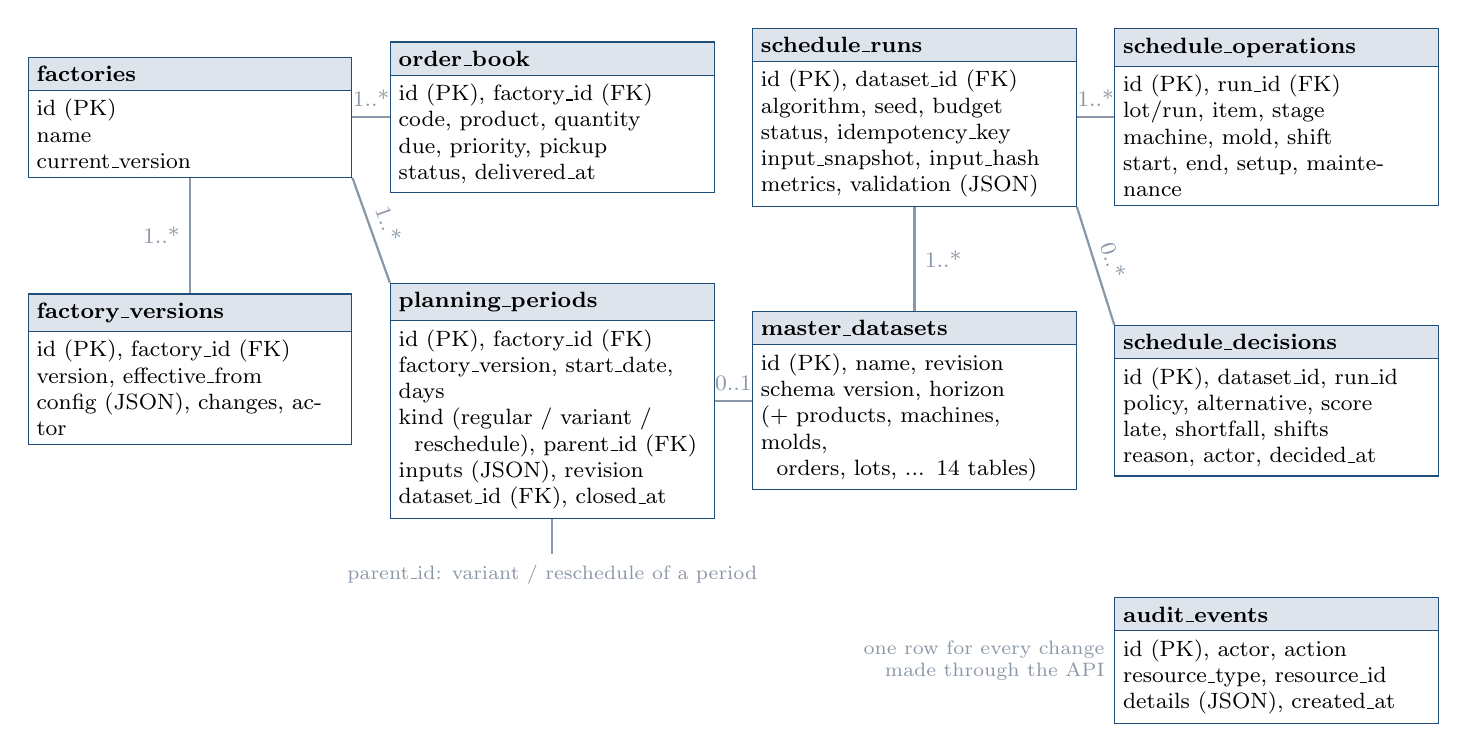
\begin{tikzpicture}[font=\footnotesize,
  ent/.style={draw=bkblue,rectangle split,rectangle split parts=2,rectangle split part fill={bkblue!15,white},
              align=left,inner sep=3pt,text width=3.9cm},
  r/.style={thick,bkgray}]
  \node[ent] (fac) at (0,0) {\textbf{factories}\nodepart{second}id (PK)\\name\\current\_version};
  \node[ent] (ver) at (0,-3.2) {\textbf{factory\_versions}\nodepart{second}id (PK), factory\_id (FK)\\version, effective\_from\\config (JSON), changes, actor};
  \node[ent] (book) at (4.6,0) {\textbf{order\_book}\nodepart{second}id (PK), factory\_id (FK)\\code, product, quantity\\due, priority, pickup\\status, delivered\_at};
  \node[ent] (per) at (4.6,-3.6) {\textbf{planning\_periods}\nodepart{second}id (PK), factory\_id (FK)\\factory\_version, start\_date, days\\kind (regular / variant /\\\ \ reschedule), parent\_id (FK)\\inputs (JSON), revision\\dataset\_id (FK), closed\_at};
  \node[ent] (ds) at (9.2,-3.6) {\textbf{master\_datasets}\nodepart{second}id (PK), name, revision\\schema version, horizon\\(+ products, machines, molds,\\\ \ orders, lots, ... 14 tables)};
  \node[ent] (run) at (9.2,0) {\textbf{schedule\_runs}\nodepart{second}id (PK), dataset\_id (FK)\\algorithm, seed, budget\\status, idempotency\_key\\input\_snapshot, input\_hash\\metrics, validation (JSON)};
  \node[ent] (op) at (13.8,0) {\textbf{schedule\_operations}\nodepart{second}id (PK), run\_id (FK)\\lot/run, item, stage\\machine, mold, shift\\start, end, setup, maintenance};
  \node[ent] (dec) at (13.8,-3.6) {\textbf{schedule\_decisions}\nodepart{second}id (PK), dataset\_id, run\_id\\policy, alternative, score\\late, shortfall, shifts\\reason, actor, decided\_at};
  \node[ent] (aud) at (13.8,-6.9) {\textbf{audit\_events}\nodepart{second}id (PK), actor, action\\resource\_type, resource\_id\\details (JSON), created\_at};
  \node[font=\scriptsize,text=bkgray,align=right,anchor=east] at (aud.west) {one row for every change\\made through the API\ };
  \draw[r] (fac) -- node[left]{1..*} (ver);
  \draw[r] (fac) -- node[above]{1..*} (book);
  \draw[r] (fac.south east) -- node[above,sloped]{1..*} (per.north west);
  \draw[r] (per) -- node[above]{0..1} (ds);
  \draw[r] (ds) -- node[right]{1..*} (run);
  \draw[r] (run) -- node[above]{1..*} (op);
  \draw[r] (run.south east) -- node[above,sloped]{0..*} (dec.north west);
  \draw[r] (per.south) -- ++(0,-0.45) node[below,font=\scriptsize,text=bkgray]{parent\_id: variant / reschedule of a period};
\end{tikzpicture}
\end{figpage}

\end{document}
